\PassOptionsToPackage{unicode=true}{hyperref} % options for packages loaded elsewhere
\PassOptionsToPackage{hyphens}{url}
%!TEX TS-program = xelatex
\documentclass[ctexart]{article}
\usepackage{lmodern}
\usepackage{amssymb,amsmath}
\usepackage{ifxetex,ifluatex}
\usepackage{fixltx2e} % provides \textsubscript
\ifnum 0\ifxetex 1\fi\ifluatex 1\fi=0 % if pdftex
  \usepackage[T1]{fontenc}
  \usepackage[utf8]{inputenc}
  \usepackage{textcomp} % provides euro and other symbols
\else % if luatex or xelatex
  \usepackage{unicode-math}
  \defaultfontfeatures{Ligatures=TeX,Scale=MatchLowercase}
\fi
% use upquote if available, for straight quotes in verbatim environments
\IfFileExists{upquote.sty}{\usepackage{upquote}}{}
% use microtype if available
\IfFileExists{microtype.sty}{%
\usepackage[]{microtype}
\UseMicrotypeSet[protrusion]{basicmath} % disable protrusion for tt fonts
}{}
\IfFileExists{parskip.sty}{%
\usepackage{parskip}
}{% else
\setlength{\parindent}{0pt}
\setlength{\parskip}{6pt plus 2pt minus 1pt}
}
\usepackage{hyperref}
\hypersetup{
            pdfborder={0 0 0},
            breaklinks=true}
\urlstyle{same}  % don't use monospace font for urls
\usepackage{color}
\usepackage{fancyvrb}
\newcommand{\VerbBar}{|}
\newcommand{\VERB}{\Verb[commandchars=\\\{\}]}
\DefineVerbatimEnvironment{Highlighting}{Verbatim}{commandchars=\\\{\}}
% Add ',fontsize=\small' for more characters per line
\newenvironment{Shaded}{}{}
\newcommand{\AlertTok}[1]{\textcolor[rgb]{1.00,0.00,0.00}{\textbf{#1}}}
\newcommand{\AnnotationTok}[1]{\textcolor[rgb]{0.38,0.63,0.69}{\textbf{\textit{#1}}}}
\newcommand{\AttributeTok}[1]{\textcolor[rgb]{0.49,0.56,0.16}{#1}}
\newcommand{\BaseNTok}[1]{\textcolor[rgb]{0.25,0.63,0.44}{#1}}
\newcommand{\BuiltInTok}[1]{#1}
\newcommand{\CharTok}[1]{\textcolor[rgb]{0.25,0.44,0.63}{#1}}
\newcommand{\CommentTok}[1]{\textcolor[rgb]{0.38,0.63,0.69}{\textit{#1}}}
\newcommand{\CommentVarTok}[1]{\textcolor[rgb]{0.38,0.63,0.69}{\textbf{\textit{#1}}}}
\newcommand{\ConstantTok}[1]{\textcolor[rgb]{0.53,0.00,0.00}{#1}}
\newcommand{\ControlFlowTok}[1]{\textcolor[rgb]{0.00,0.44,0.13}{\textbf{#1}}}
\newcommand{\DataTypeTok}[1]{\textcolor[rgb]{0.56,0.13,0.00}{#1}}
\newcommand{\DecValTok}[1]{\textcolor[rgb]{0.25,0.63,0.44}{#1}}
\newcommand{\DocumentationTok}[1]{\textcolor[rgb]{0.73,0.13,0.13}{\textit{#1}}}
\newcommand{\ErrorTok}[1]{\textcolor[rgb]{1.00,0.00,0.00}{\textbf{#1}}}
\newcommand{\ExtensionTok}[1]{#1}
\newcommand{\FloatTok}[1]{\textcolor[rgb]{0.25,0.63,0.44}{#1}}
\newcommand{\FunctionTok}[1]{\textcolor[rgb]{0.02,0.16,0.49}{#1}}
\newcommand{\ImportTok}[1]{#1}
\newcommand{\InformationTok}[1]{\textcolor[rgb]{0.38,0.63,0.69}{\textbf{\textit{#1}}}}
\newcommand{\KeywordTok}[1]{\textcolor[rgb]{0.00,0.44,0.13}{\textbf{#1}}}
\newcommand{\NormalTok}[1]{#1}
\newcommand{\OperatorTok}[1]{\textcolor[rgb]{0.40,0.40,0.40}{#1}}
\newcommand{\OtherTok}[1]{\textcolor[rgb]{0.00,0.44,0.13}{#1}}
\newcommand{\PreprocessorTok}[1]{\textcolor[rgb]{0.74,0.48,0.00}{#1}}
\newcommand{\RegionMarkerTok}[1]{#1}
\newcommand{\SpecialCharTok}[1]{\textcolor[rgb]{0.25,0.44,0.63}{#1}}
\newcommand{\SpecialStringTok}[1]{\textcolor[rgb]{0.73,0.40,0.53}{#1}}
\newcommand{\StringTok}[1]{\textcolor[rgb]{0.25,0.44,0.63}{#1}}
\newcommand{\VariableTok}[1]{\textcolor[rgb]{0.10,0.09,0.49}{#1}}
\newcommand{\VerbatimStringTok}[1]{\textcolor[rgb]{0.25,0.44,0.63}{#1}}
\newcommand{\WarningTok}[1]{\textcolor[rgb]{0.38,0.63,0.69}{\textbf{\textit{#1}}}}
\usepackage{graphicx,grffile}
\makeatletter
\def\maxwidth{\ifdim\Gin@nat@width>\linewidth\linewidth\else\Gin@nat@width\fi}
\def\maxheight{\ifdim\Gin@nat@height>\textheight\textheight\else\Gin@nat@height\fi}
\makeatother
% Scale images if necessary, so that they will not overflow the page
% margins by default, and it is still possible to overwrite the defaults
% using explicit options in \includegraphics[width, height, ...]{}
\setkeys{Gin}{width=\maxwidth,height=\maxheight,keepaspectratio}
\setlength{\emergencystretch}{3em}  % prevent overfull lines
\providecommand{\tightlist}{%
  \setlength{\itemsep}{0pt}\setlength{\parskip}{0pt}}
\setcounter{secnumdepth}{0}
% Redefines (sub)paragraphs to behave more like sections
\ifx\paragraph\undefined\else
\let\oldparagraph\paragraph
\renewcommand{\paragraph}[1]{\oldparagraph{#1}\mbox{}}
\fi
\ifx\subparagraph\undefined\else
\let\oldsubparagraph\subparagraph
\renewcommand{\subparagraph}[1]{\oldsubparagraph{#1}\mbox{}}
\fi

% set default figure placement to htbp
\makeatletter
\def\fps@figure{htbp}
\makeatother


\date{}

\begin{document}

\hypertarget{header-n0}{%
\section{一、实验目的}\label{header-n0}}

\begin{itemize}
\item
  实现原始的批处理操作系统
\end{itemize}

\begin{itemize}
\item
  学习内核从外存加载和结束用户程序的方法
\item
  学习使用BIOS中断
\end{itemize}

\hypertarget{header-n13}{%
\section{二、实验要求}\label{header-n13}}

\begin{itemize}
\item
  实现监控程序,显示必要的提示信息后,从引导盘的特定扇区加载一个他人开发的COM格式的可执行程序到指定的内存位置,然后启动这个程序,实现操作系统执行用户程序这一项基本功能。
\item
  设计四个有输出的用户可执行程序,分别在屏幕1/4区域动态输出字符,如将用字符`A'从屏幕左边某行位置45度角下斜射出,保持一个可观察的适当速度直线运动,碰到屏幕相应1/4区域的边后产生反射,改变方向运动,如此类推,不断运动;在此基础上,增加你的个性扩展,如同时控制两个运动的轨迹,或炫酷动态变色,个性画面,如此等等,自由不限。还要在屏幕某个区域特别的方式显示你的学号姓名等个人信息。
\item
  修改参考原型代码,允许键盘输入,用于指定运行这四个有输出的用户可执行程序之一,要确保系统执行代码不超过512字节,以便放在引导扇区。
\item
  自行组织映像盘的空间存放四个用户可执行程序。
\end{itemize}

\hypertarget{header-n922}{%
\section{三、实验环境}\label{header-n922}}

与实验一大致相同:

主机操作系统:Mac OS 10.12

编辑器:Vim 8.0.1400、VS Code 1.21.0

汇编器:Nasm 2.13.02

虚拟机、调试器:Bochs 2.6.9

版本控制:Git 2.15.1

自动构建:GNU Make 3.8.1

\hypertarget{header-n21}{%
\section{四、实验方案}\label{header-n21}}

\hypertarget{header-n22}{%
\subsection{(一)、基础要求部分}\label{header-n22}}

\hypertarget{header-n310}{%
\subsubsection{1、监控程序的启动}\label{header-n310}}

与实验一相同:监控程序放入软盘第0号扇区,并将扇区最后两个字节写人0x55,0xAA后,即可被BIOS加载到0x7C00处。启动后,监控程序将使用BIOS
0x10中断打印出开机欢迎字符,并提示用户输入。监控程序使用BIOS
0x16号中断的0号功能(AH=0)阻塞读取键盘缓冲区,获得用户输入,根据输入判断要加载哪个用户程序。

\hypertarget{header-n324}{%
\subsubsection{2、加载用户程序}\label{header-n324}}

\hypertarget{header-n326}{%
\paragraph{(1) 编写20h,21h号中断,设置PSP}\label{header-n326}}

监控程序在加载用户程序必须做相关操作,而不能像提供的示例代码那样直接jmp到用户程序中,才能确保用户程序能够正确返回监控程序。

一个较为简便的方法是使用call指令,call指令能够将当前指令的下一条指令的CS、IP压栈,在用户程序中调用ret指令就可以返回监控程序。但这样做的局限性是:用户程序可能对栈进行很多操作,这些操作中一旦破坏了栈顶的CS、IP,用户程序就不能返回监控程序了。

因此,我选择使用了真实的DOS系统的解决方法:在加载用户程序前,首先在用户程序载入地址(本实验中选择0xA100)的前256个字节处(0xA000)写入PSP(程序段前缀)。程序段前缀包含很多信息,其中我选择性地写入了和返回操作系统有关的:在0x00处写入CDh
20h(int 20h的机器码),在0x0A处写入返回地址的IP、CS。

在真实的DOS系统中,程序有两种方法返回DOS:一是通过ret指令返回到PSP中的int
20h指令,二是调用给你21h中断的4ch功能。这两个中断都是DOS系统中断,在我的操作系统中我对它们进行了实现,代码如下:

\begin{verbatim}
interrupt_20h:						;这里20h中断实际上是使用21h中断来工作
      mov ah, 4ch
interrupt_21h:
      cmp ah, 4ch					;判断功能号是不是4ch
      jnz panic_21h_func_not_impl	;如果不是,陷入kernel panic
      jmp dword[0xA00A]				;如果是,使用jmp跳回psp中的返回地址
      iret
panic_21h_func_not_impl:			;提示只实现了4ch号功能
      print_string panic_21h_msg, paini_21h_len, 0, 0
      jmp $
\end{verbatim}

通过这种方法,我的操作系统拥有了从正确的DOS程序返回的兼容性。

\hypertarget{header-n472}{%
\paragraph{(2)安装中断}\label{header-n472}}

中断向量表是从内存0号单元开始1k字节的内存空间,最多存放256个中断服务程序的入口地址,安装N号中断中断的方法就是将中断服务程序的IP、CS写入0000:{[}4N{]},
0000:{[}4N + 2{]}处。

\hypertarget{header-n405}{%
\paragraph{(2) 加载用户程序到内存并跳转}\label{header-n405}}

实现加载用户程序到内存使用的是BIOS
13H号中断的2号功能:分别将驱动器、柱面、磁头、扇区号写入dl, ch, dh,
cl寄存器,在ah中写入读取的扇区数量,并在bx中写入要把扇区载入到的内存地址,调用中断即可实现加载磁盘指定位置的扇区到指定内存。

在本实验中,驱动器、柱面、磁头号均为0, 第N个用户程序被放在第2N +
1个扇区,并最多占用两个扇区,因此设置al为2,载入的地址是bx = 0xA100。

最后,监控程序首先使用pusha保护了当前寄存器值,然后通过jmp指令启动了用户程序。

\hypertarget{header-n314}{%
\subsubsection{3、用户程序(屏幕1/4区域弹射字符)的实现}\label{header-n314}}

\hypertarget{header-n439}{%
\paragraph{(1)响应键盘输入}\label{header-n439}}

用户程序需要在正常执行过程中响应键盘输入,随时准备返回操作系统。这一功能是通过BIOS的0x16中断的1号功能实现的,该功能检测当前键盘是否按下并依此设置ZF为0(无按下)或1(有按下)。如果有按下,用户程序又要调用0x16中断的0号功能,通过读取输入清空键盘缓冲区,然后判断该按键的ASCII码(存在al中),进行判断处理。

\hypertarget{header-n446}{%
\paragraph{(2)屏幕区域划分}\label{header-n446}}

本实验使用了NASM的macro功能,将4个弹射字符程序共同的部分写为一个macro,这个macro接收4个参数,分布表示x坐标的下边界和上边界,y坐标的下边界和上边界。在4个asm文件中分别使用不同参数调用这个宏,从而实现了4个不同的用户程序。

\hypertarget{header-n459}{%
\paragraph{(3)返回操作系统}\label{header-n459}}

本实验中按下ESC键(27)会使得用户程序退出。上文已经提到,本操作系统中的用户程序可以使用标准的DOS程序返回方法(ret到PSP开头的int
20h指令或调用int 21h的4ch功能)。

\hypertarget{header-n434}{%
\subsection{(二)、扩展创新部分}\label{header-n434}}

\hypertarget{header-n492}{%
\subsubsection{1、代码改进和《贪吃蛇》游戏的实现}\label{header-n492}}

本实验中,我首先改进了实验一中的弹射字符程序的算法,改为使用当前速度方向Vn和当前位置Pn来确定下一时刻字符的位置(公式1)。每次移动字符后判断是否碰到边界,如果碰到只需使对应速度分量的方向取反即可。

\[P_{n+1} = P_{n} + V_n\space\space\space\space\space\space\space\space\space\space(1)\]

使用该算法,实验一中的程序缩减了80行的代码。

除此之外,还实现了显示固定长度的字符长串功能。这一功能是通过使用数组保存之前字符的位置,结合nasm的\%rep宏和movsb指令实现的。

最后,在能够显示固定长度的字符长串的基础上,我制作了《贪吃蛇》游戏。游戏中玩家能够控制一个初试长度为2的''蛇``(用字符*组成的长串表示),用按键wasd控制蛇向上、向左、向下、向右运动。屏幕上会出现一个随机生成的''果实``(用白底字符o表示),蛇每吃到一个果实长度就会加一,如果蛇碰到屏幕边缘就会游戏结束。程序的流程图如下:

\begin{figure}
\centering
\includegraphics{/Users/lixinrui/Downloads/Untitled Diagram.png}
\caption{}
\end{figure}

这里用到的随机数程序是原理是,通过调用BIOS
0x1A号中断,读取当前时钟计数。然后与 0x11ee
相与运算后(根据本实验实际需要计算出的值,防止除法商太大溢出)使用div指令与数字N进行运算,就可以在ah中得到一个0到N-1的随机数。

\hypertarget{header-n511}{%
\subsubsection{2、自动处理任意多用户程序的Makefile}\label{header-n511}}

在实验二中有4个以上的用户程序要编译,写入磁盘镜像,逐一手动写入的方法显得耗时耗力,更为不可取了。因此我改进了实验一中的Makefile,使之能够找到同一目录下所有以user开头的asm文件,将他们自动编译,并按照文件名排序逐一写入到软盘镜像。

改进部分的代码如下:

\begin{Shaded}
\begin{Highlighting}[]
\KeywordTok{include}\NormalTok{ gmsl								}\CommentTok{#用到plus函数}
\DataTypeTok{disk_index }\CharTok{=}\StringTok{ 1								#计数是第几个用户程序}
\DataTypeTok{SHELL}\CharTok{=}\StringTok{/bin/bash							}
\DataTypeTok{AS }\CharTok{=}\StringTok{ nasm}
\DataTypeTok{ASFLAG }\CharTok{=}\StringTok{ -f bin}
\DataTypeTok{user_src }\CharTok{=}\StringTok{ }\CharTok{$(}\KeywordTok{sort}\StringTok{ }\CharTok{$(}\KeywordTok{wildcard}\StringTok{ user*.asm}\CharTok{))}\StringTok{	#记录目录下所有用户程序源码文件}
\DataTypeTok{user_bin }\CharTok{=}\StringTok{ }\CharTok{$(}\DataTypeTok{user_src}\ErrorTok{:}\DataTypeTok{.asm}\ErrorTok{=}\DataTypeTok{.o}\CharTok{)}\StringTok{				#用户程序}
\DecValTok{user%.o :}\DataTypeTok{ user%.asm common.asm				}\CommentTok{#生成每个用户程序的规则}
	\CharTok{$(}\DataTypeTok{AS}\CharTok{)} \CharTok{$(}\DataTypeTok{ASFLAG}\CharTok{)} \CharTok{$<}\NormalTok{ -o }\CharTok{$@}
\DataTypeTok{kernal_src }\CharTok{=}\StringTok{ myos1.asm						}
\DataTypeTok{kernal_bin }\CharTok{=}\StringTok{ }\CharTok{$(}\DataTypeTok{kernal_src}\ErrorTok{:}\DataTypeTok{.asm}\ErrorTok{=}\DataTypeTok{.o}\CharTok{)}\StringTok{			}
\DecValTok{kernal :}\DataTypeTok{ }\CharTok{$(}\DataTypeTok{kernal_src}\CharTok{)}\DataTypeTok{	}
	\CharTok{$(}\DataTypeTok{AS}\CharTok{)} \CharTok{$(}\DataTypeTok{ASFLAG}\CharTok{)} \CharTok{$(}\DataTypeTok{kernal_src}\CharTok{)}\NormalTok{ -o }\CharTok{$(}\DataTypeTok{kernal_bin}\CharTok{)}
\DataTypeTok{floppyfile }\CharTok{=}\StringTok{ disk.img}
\DecValTok{clean_disk:}\DataTypeTok{									}\CommentTok{#首先生成空白软盘}
\NormalTok{	dd if=/dev/zero of=}\CharTok{$(}\DataTypeTok{floppyfile}\CharTok{)}\NormalTok{ bs=512 count=2880}
\DecValTok{write_kernal:}\DataTypeTok{ clean_disk kernal				}\CommentTok{#然后写入控制程序}
\NormalTok{	dd if=}\CharTok{$(}\DataTypeTok{kernal_bin}\CharTok{)}\NormalTok{ of=}\CharTok{$(}\DataTypeTok{floppyfile}\CharTok{)}\NormalTok{ conv=notrunc}
\KeywordTok{define}\NormalTok{ DO_write								}\CommentTok{#在下面被调用}
\NormalTok{dd }\DataTypeTok{if}\CharTok{=$(}\KeywordTok{strip}\StringTok{ }\CharTok{$(}\DataTypeTok{1}\CharTok{))}\StringTok{ of=}\CharTok{$(}\DataTypeTok{floppyfile}\CharTok{)}\StringTok{ bs=1024 seek=}\CharTok{$(}\KeywordTok{strip}\StringTok{ }\CharTok{$(}\DataTypeTok{disk_index}\CharTok{))}\StringTok{ conv=notrunc}
\CharTok{$(}\KeywordTok{eval}\StringTok{ disk_index = }\CharTok{$(}\KeywordTok{call}\StringTok{ plus}\KeywordTok{,}\CharTok{$(}\DataTypeTok{disk_index}\CharTok{)}\KeywordTok{,}\StringTok{1}\CharTok{))}

\KeywordTok{endef}
\DecValTok{write_all_progs:}\DataTypeTok{ write_kernal }\CharTok{$(}\DataTypeTok{user_bin}\CharTok{)}\DataTypeTok{	}\CommentTok{#通过foreach函数逐一将用户程序写入软盘}
	\CharTok{$(}\KeywordTok{foreach}\StringTok{ user_prog}\KeywordTok{,}\StringTok{ }\CharTok{$(}\DataTypeTok{user_bin}\CharTok{)}\KeywordTok{,}\StringTok{ }\CharTok{$(}\KeywordTok{call}\StringTok{ DO_write}\KeywordTok{,}\StringTok{ }\CharTok{$(}\DataTypeTok{user_prog}\CharTok{)))}
\end{Highlighting}
\end{Shaded}

\hypertarget{header-n152}{%
\subsection{四、实验过程和结果}\label{header-n152}}

在VS
Code编辑器中写好监控程序myos1.asm和user1.asm到user5.asm五个用户程序后,直接在屏幕下方的内置Terminal中输入
make
bochs,各个程序的编辑,写入软盘的过程就很快完成了,bochs虚拟机立即加载软盘镜像启动了虚拟机。

\begin{figure}
\centering
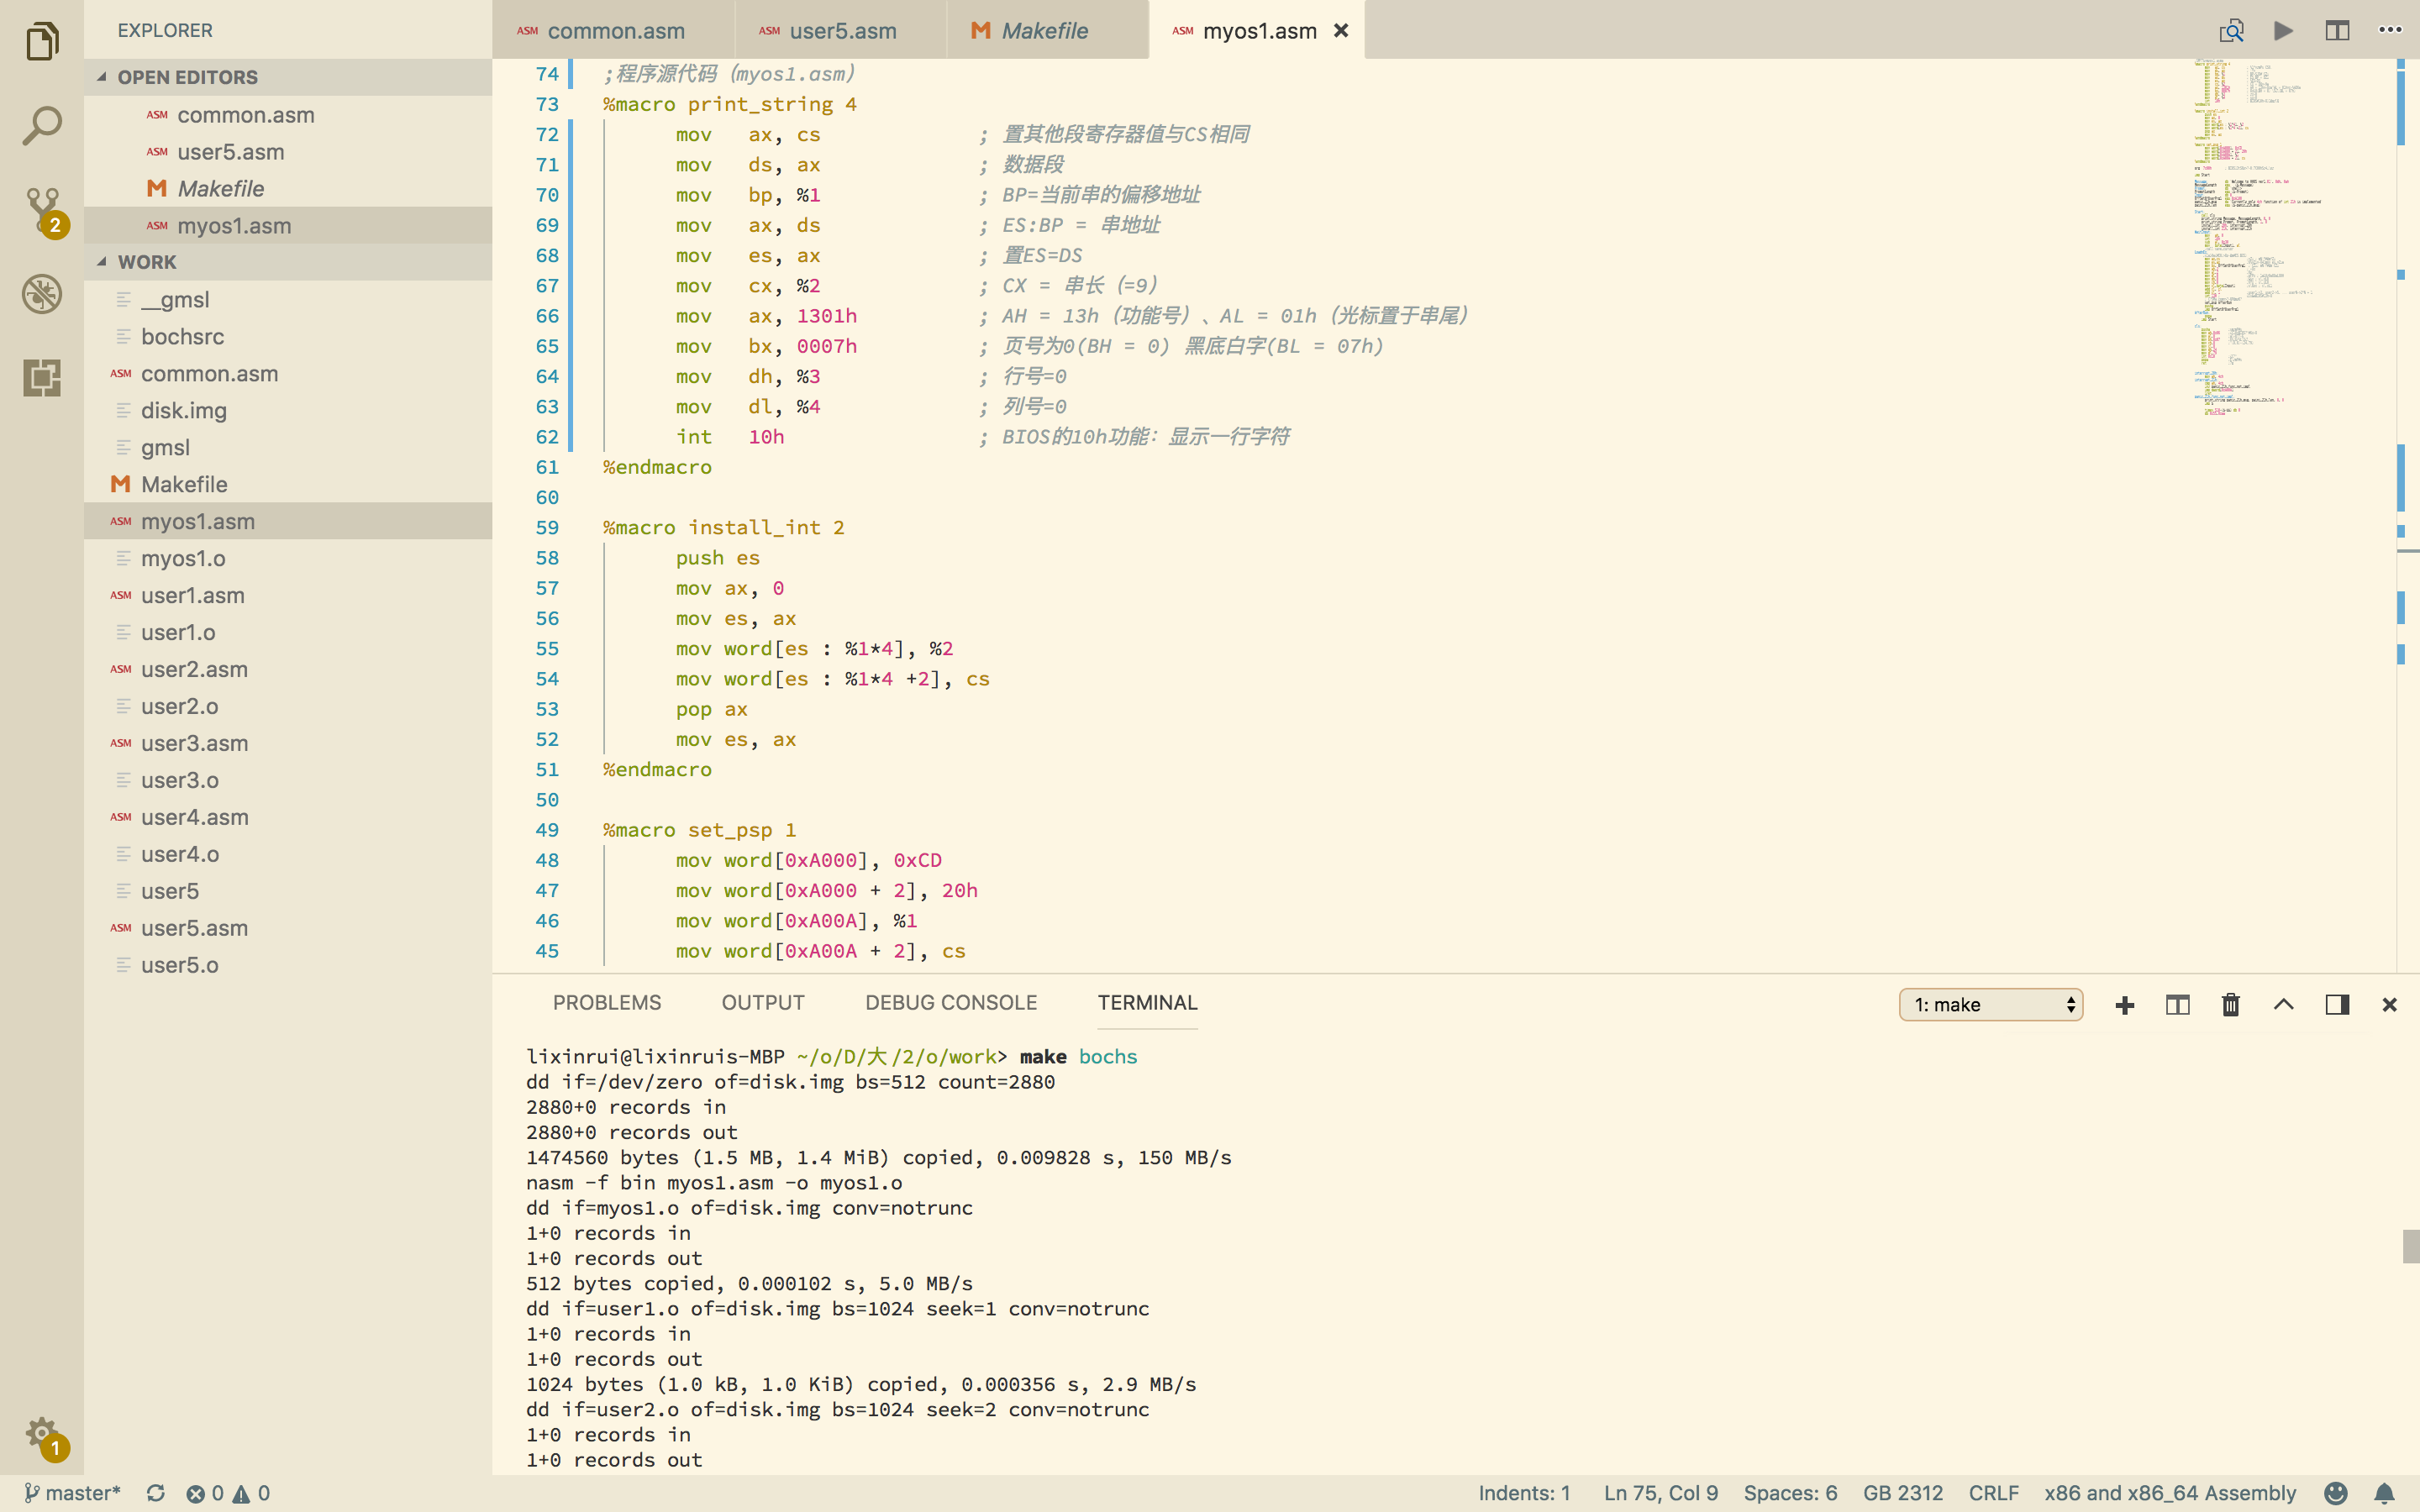
\includegraphics{/Users/lixinrui/onedrive/Documents/大学课程/2018操作系统实验/os_lab2/report/vsc.png}
\caption{}
\end{figure}

(图一:编辑和运行环境)

在VS
Code内置Terminal中输入c使虚拟机继续执行,操作系统首先进入了监控程序界面:

\begin{figure}
\centering
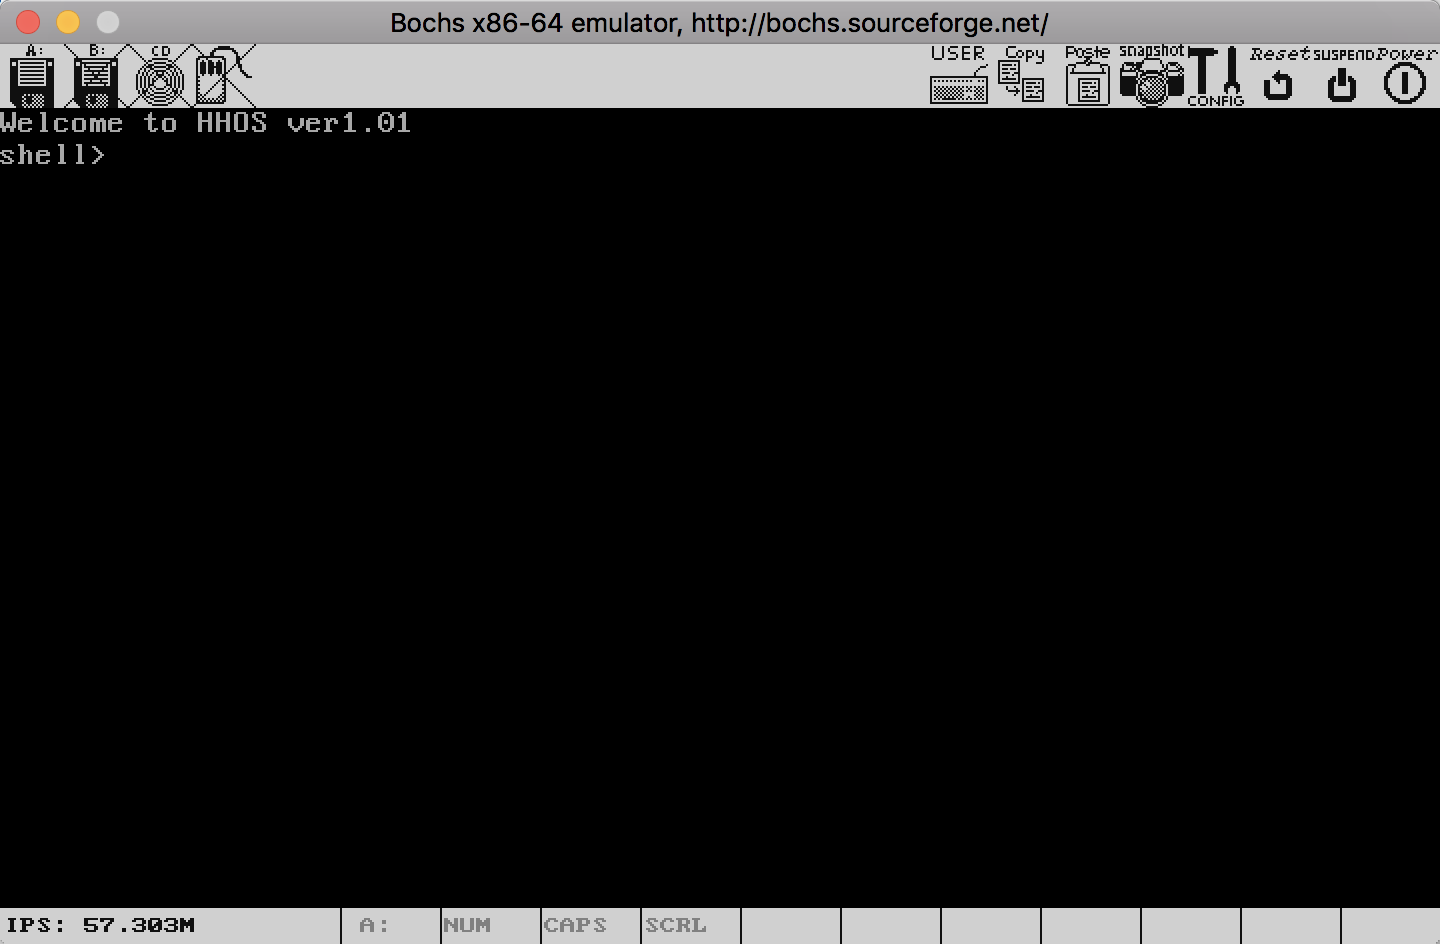
\includegraphics{/Users/lixinrui/onedrive/Documents/大学课程/2018操作系统实验/os_lab2/report/welcome.png}
\caption{}
\end{figure}

(图二:监控程序界面)

输入数字1到5可以选择执行用户程序,执行完一个程序后按下ESC回到监控程序并切换到下一个。

1到4依次是在屏幕左上到左下顺时针4个区域弹射固定长度的字符长串的程序,下面4张图片将依次演示:

\begin{figure}
\centering
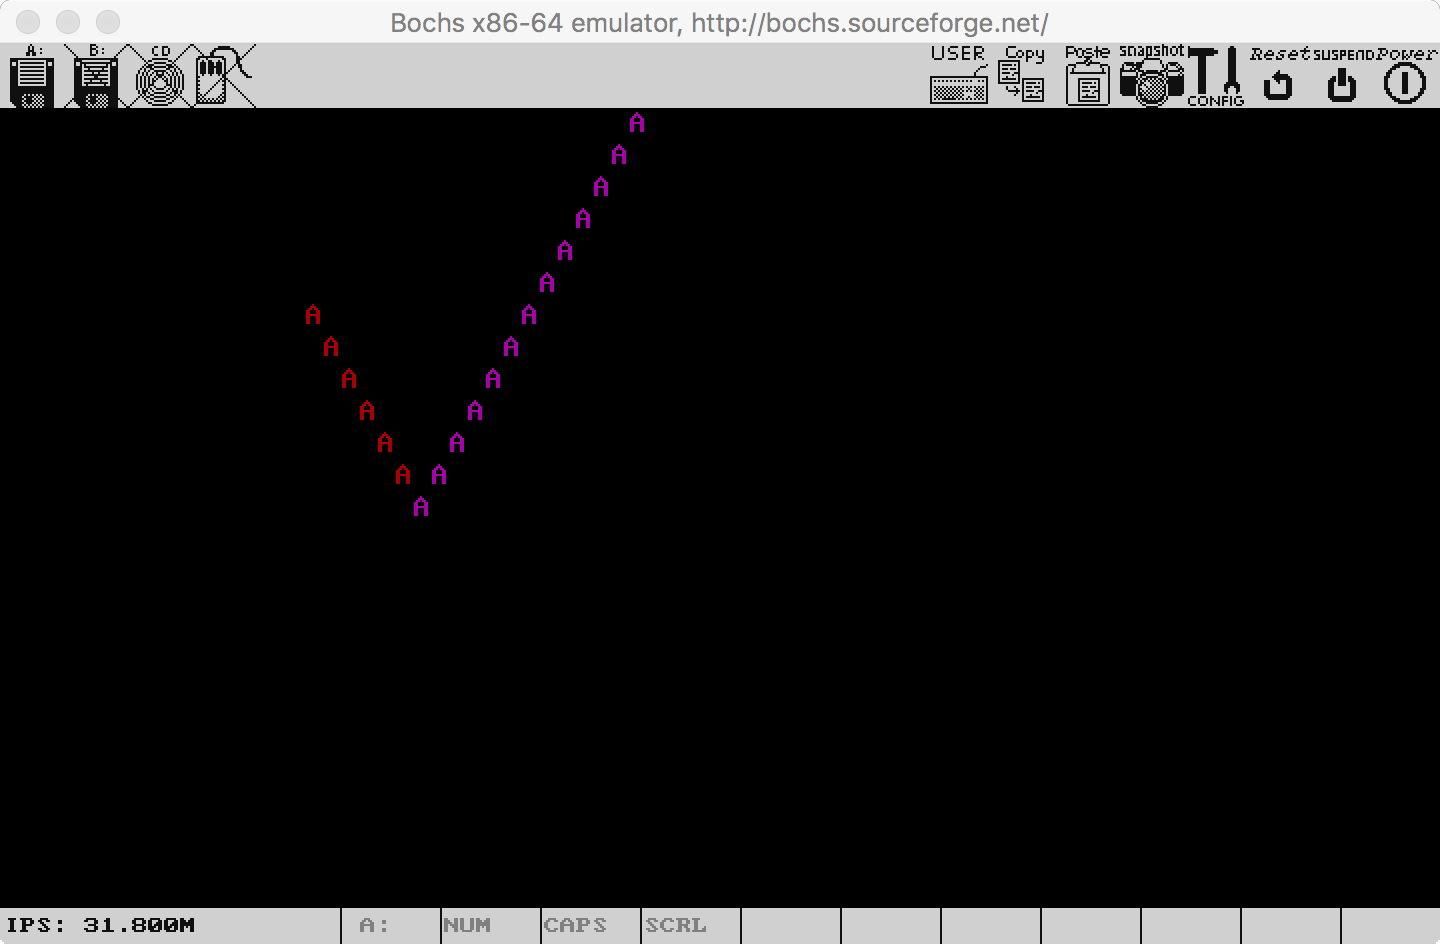
\includegraphics{/Users/lixinrui/onedrive/Documents/大学课程/2018操作系统实验/os_lab2/report/prog1.png}
\caption{}
\end{figure}

(图三:在左上角运动的用户程序一)

\begin{figure}
\centering
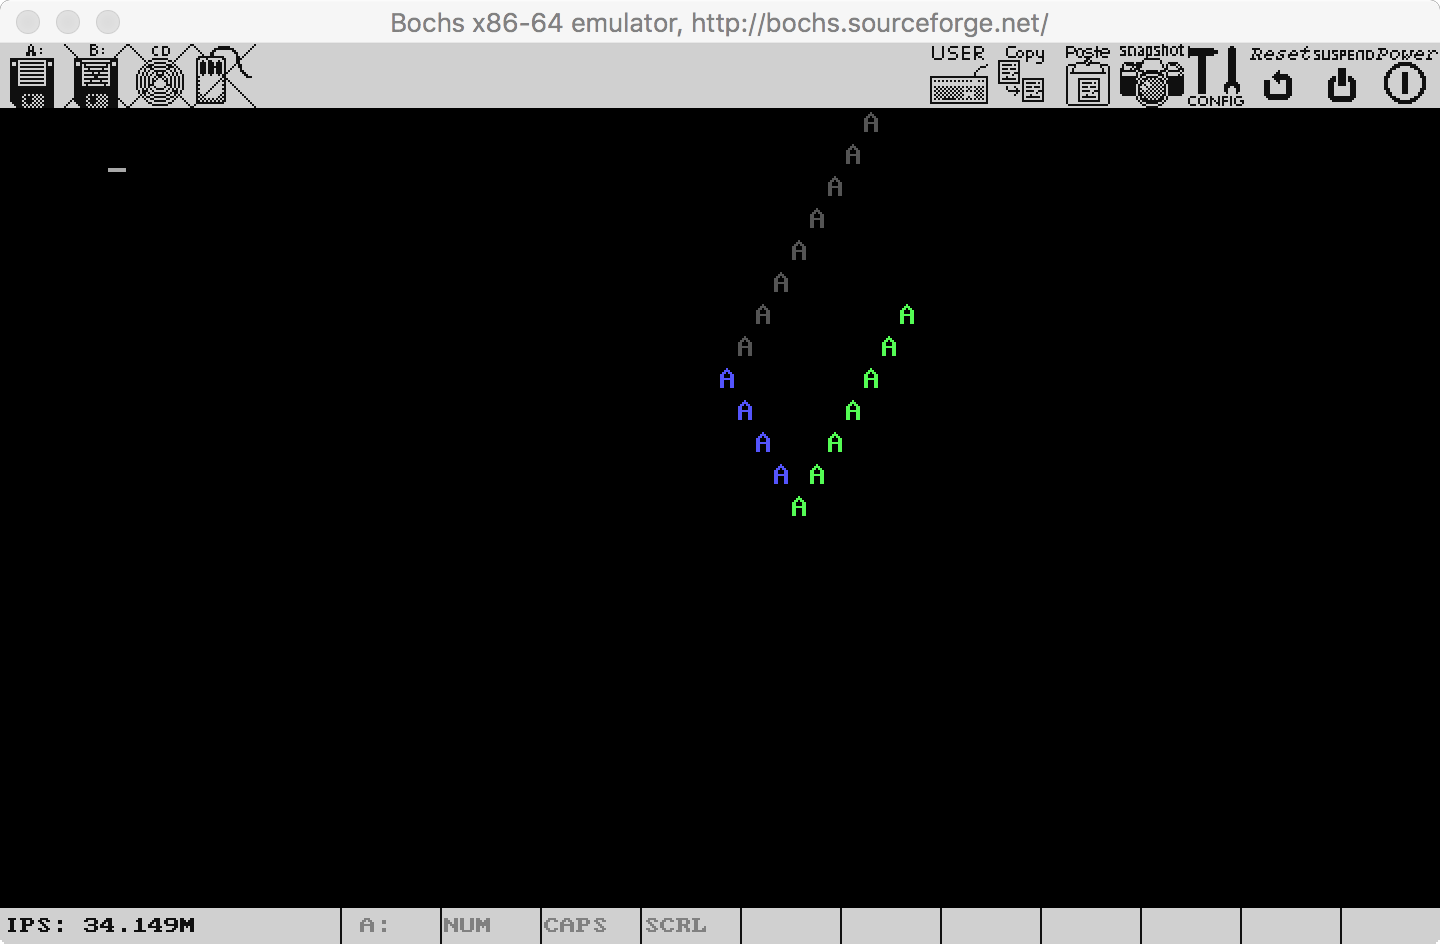
\includegraphics{/Users/lixinrui/onedrive/Documents/大学课程/2018操作系统实验/os_lab2/report/prog2.png}
\caption{}
\end{figure}

(图四:在右上角运动的用户程序二)

\begin{figure}
\centering
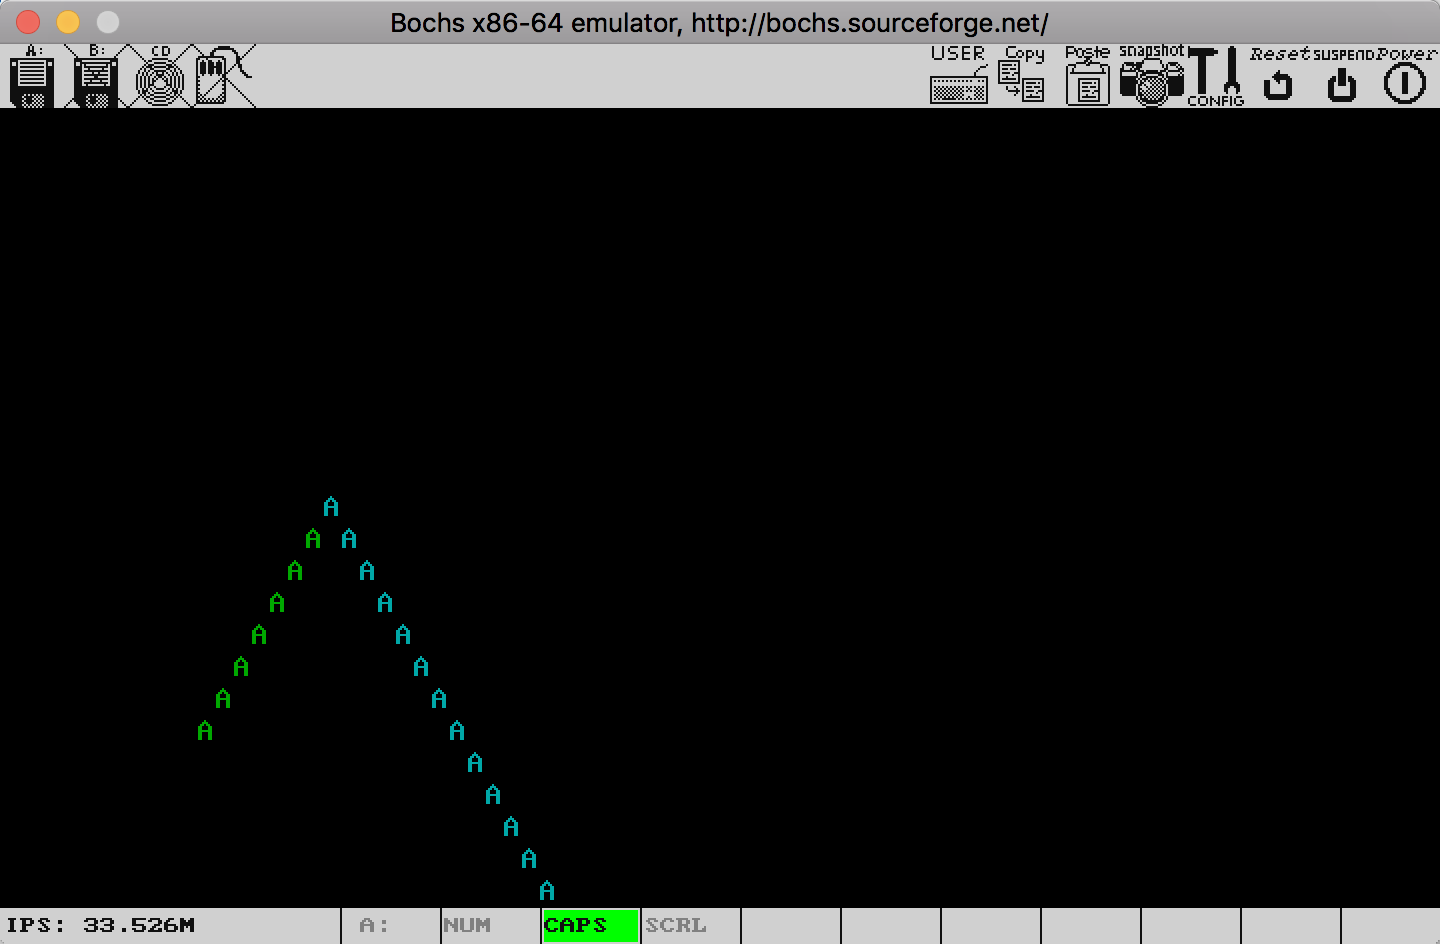
\includegraphics{/Users/lixinrui/onedrive/Documents/大学课程/2018操作系统实验/os_lab2/report/prog3.png}
\caption{}
\end{figure}

(图五:在左下角运动的用户程序三)

\begin{figure}
\centering
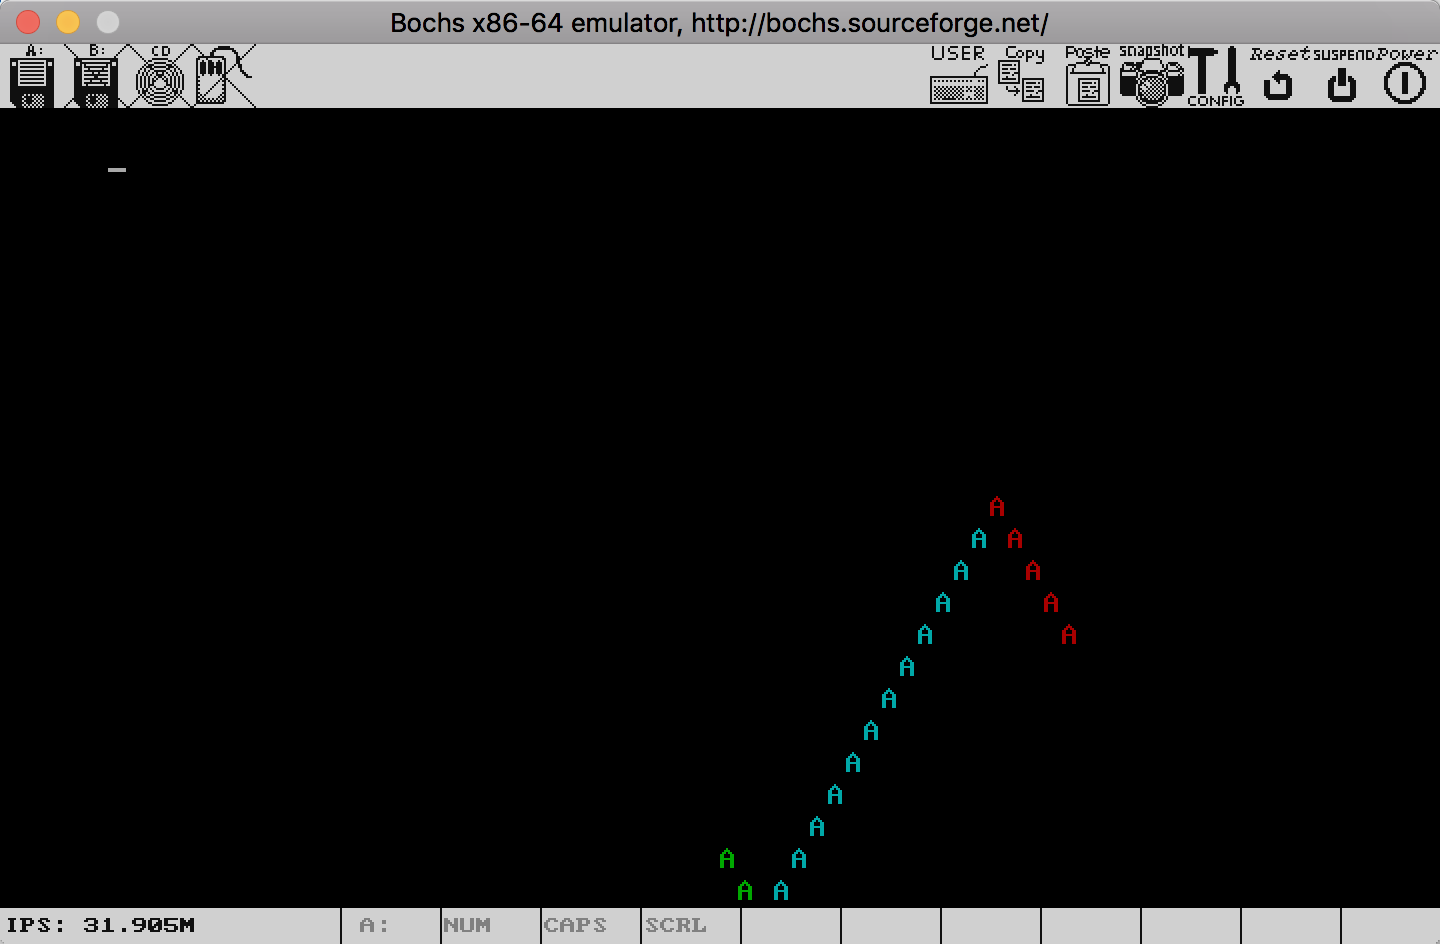
\includegraphics{/Users/lixinrui/onedrive/Documents/大学课程/2018操作系统实验/os_lab2/report/prog4.png}
\caption{}
\end{figure}

(图六:在右下角运动的用户程序四)

最后是展示《贪吃蛇》游戏截图,另有游戏录像在screen\_record文件夹中。

\begin{figure}
\centering
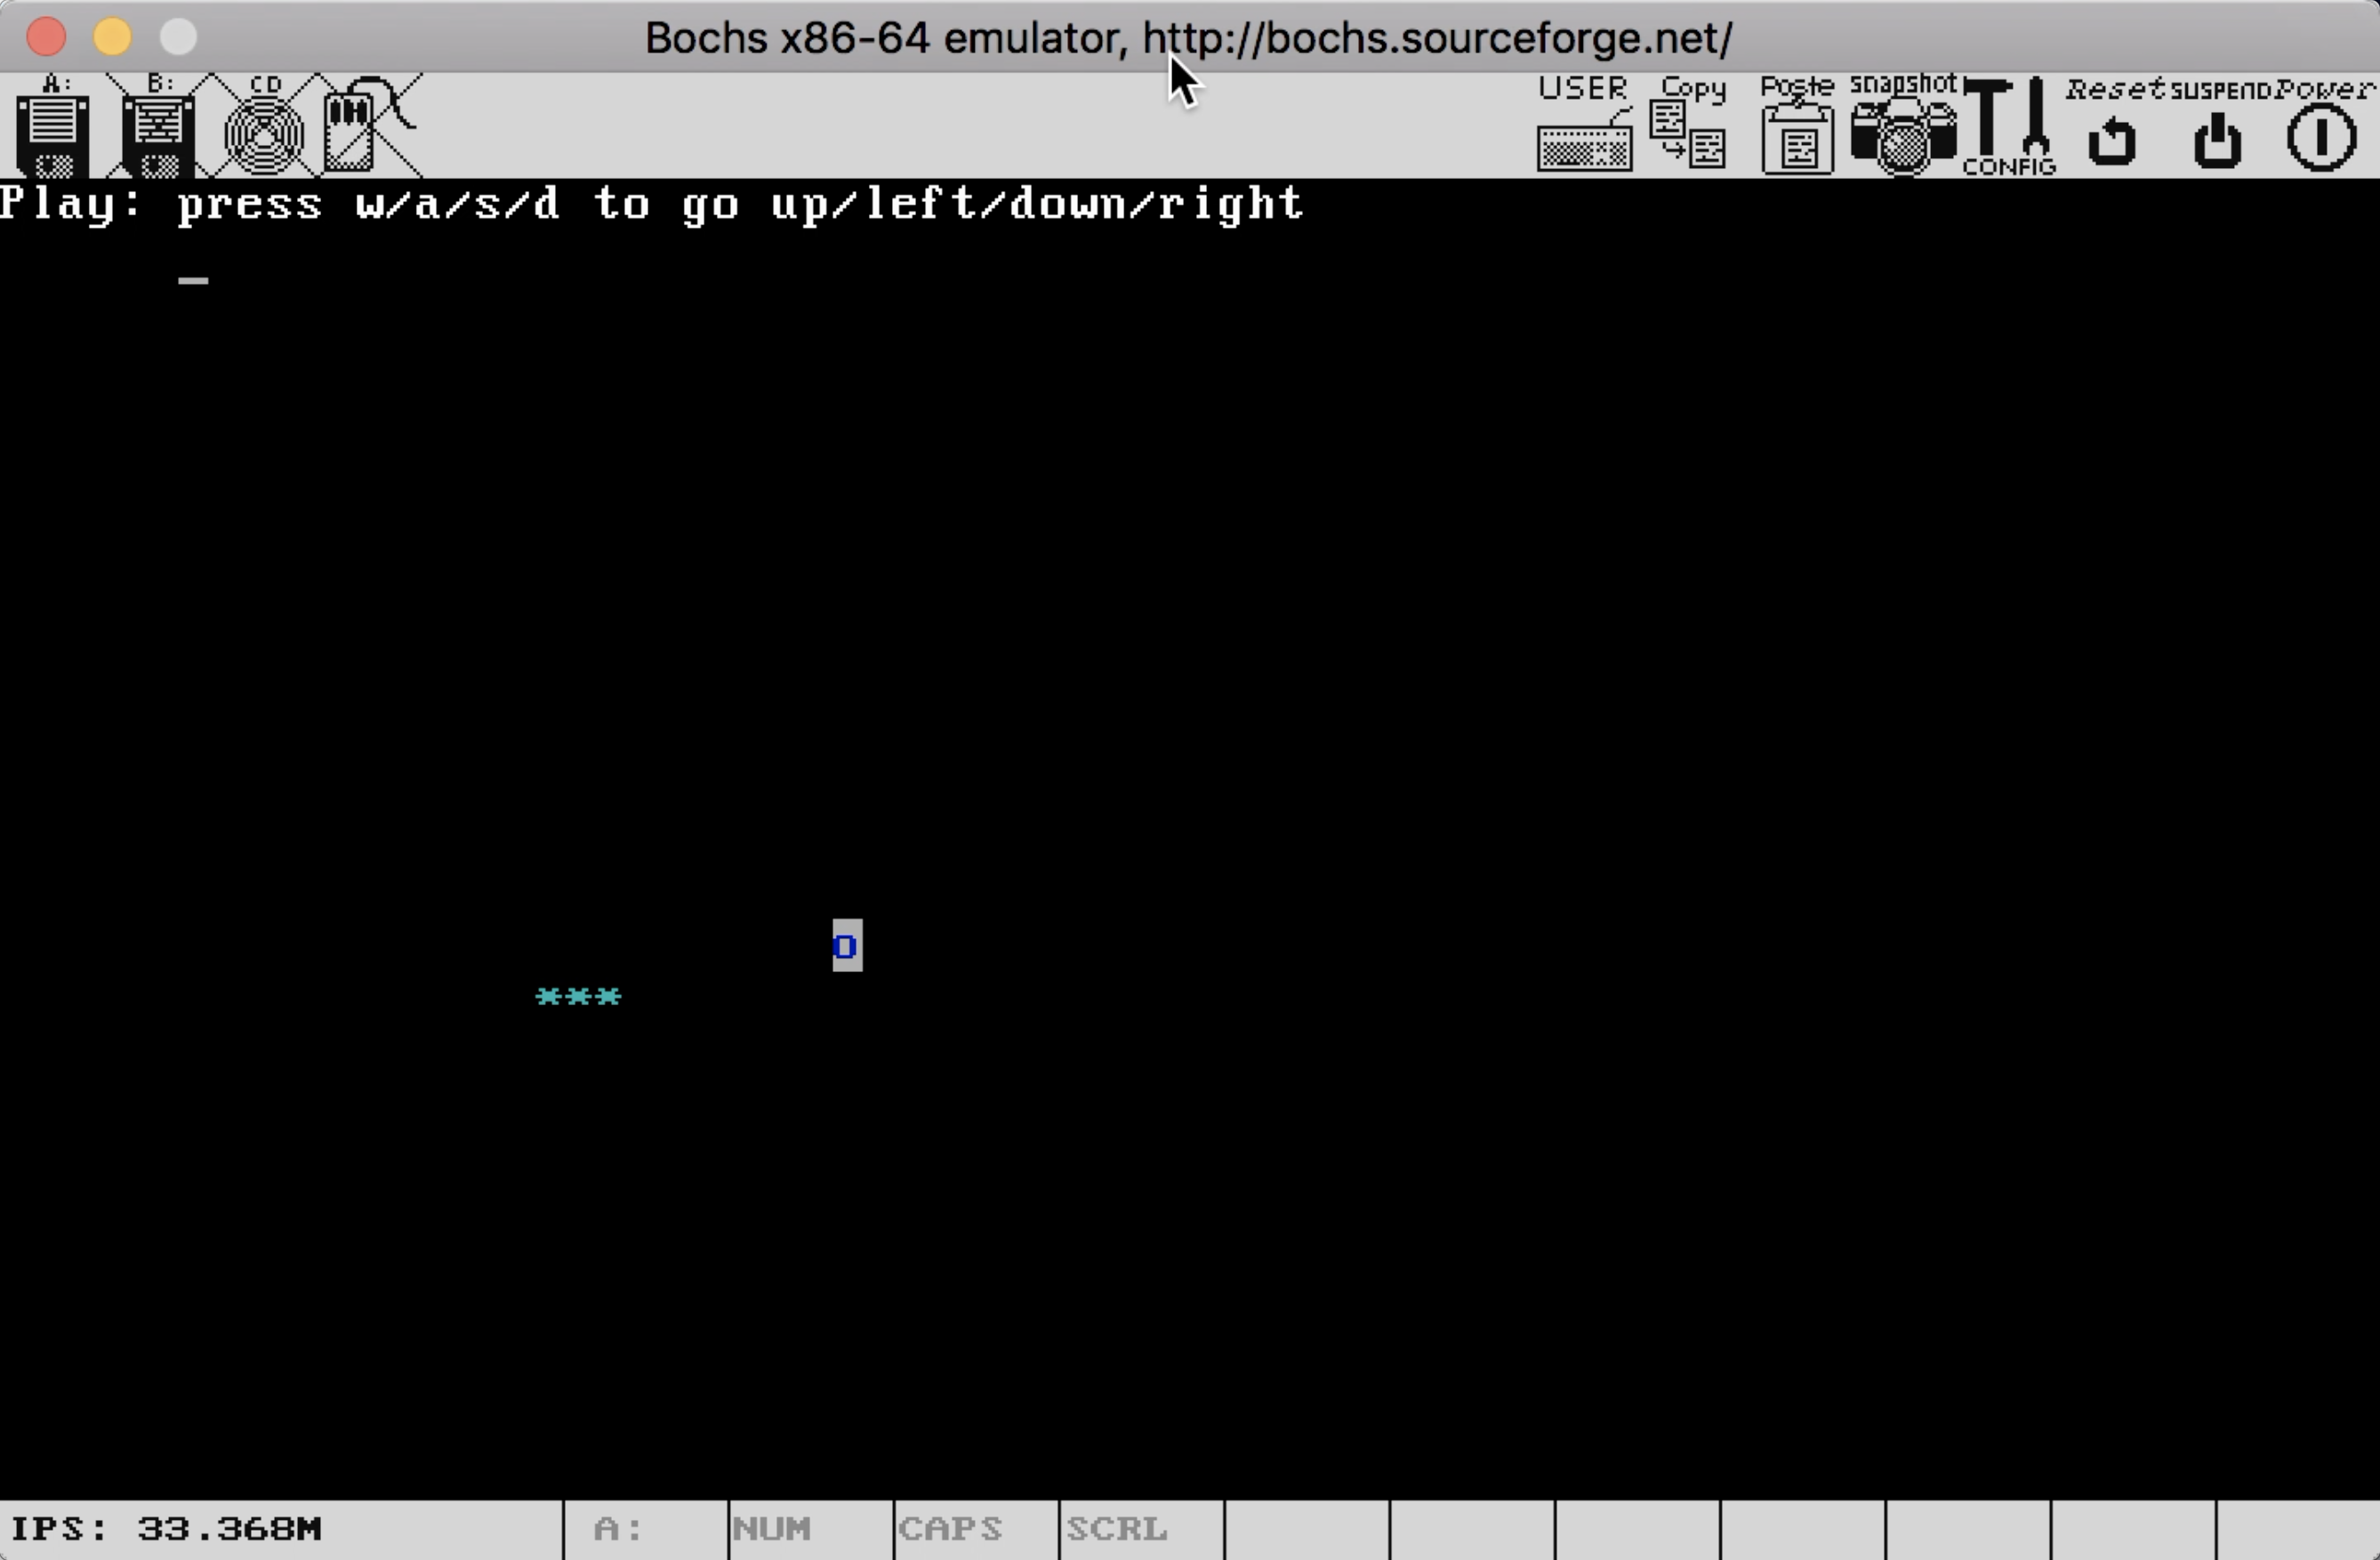
\includegraphics{/Users/lixinrui/onedrive/Documents/大学课程/2018操作系统实验/os_lab2/report/py1.png}
\caption{}
\end{figure}

(图七:当前蛇长度为3)

\begin{figure}
\centering
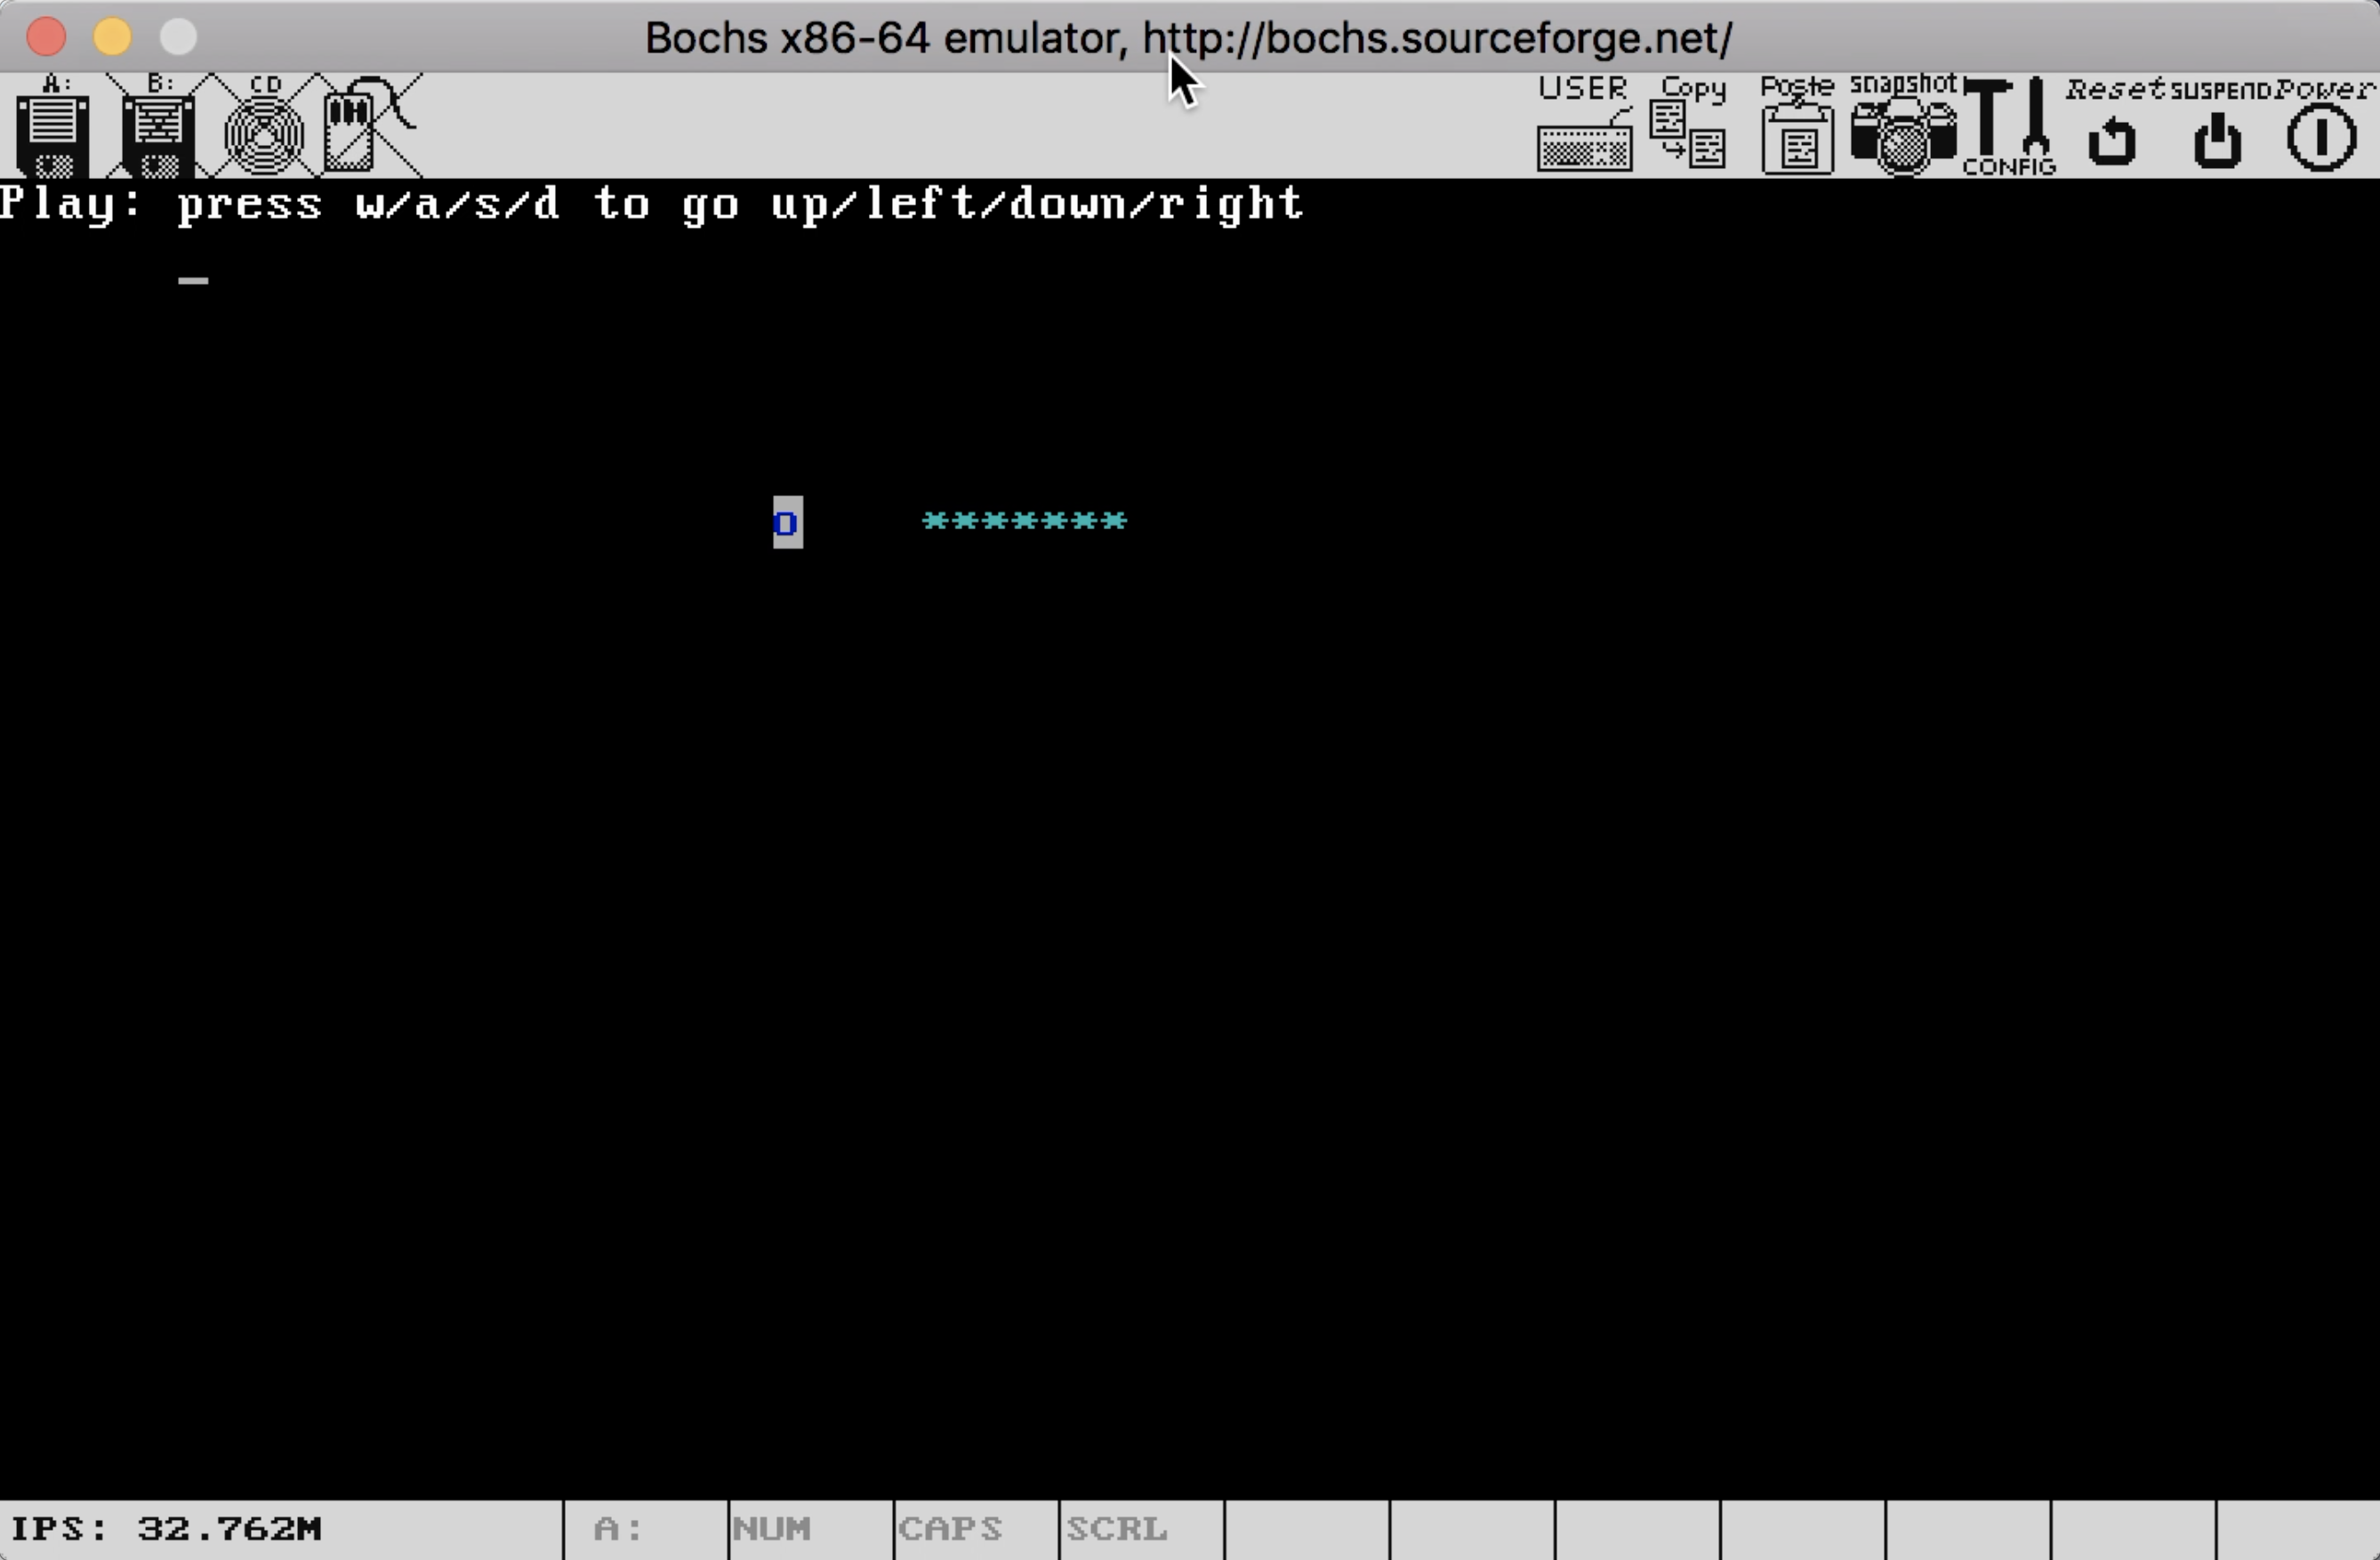
\includegraphics{/Users/lixinrui/onedrive/Documents/大学课程/2018操作系统实验/os_lab2/report/py2.png}
\caption{}
\end{figure}

(图八:当前蛇长度为7)

\hypertarget{header-n1125}{%
\subsection{五、实验总结}\label{header-n1125}}

本周的操作系统实验花费了我不少的心血,学到了不少的新东西。在开始研究和编写代码之前,我首先翻看完了200多页的Nasm文档学会了Nasm中宏的写法,在本次实验中给了我很大的帮助。之后我开始编写新的Makefile之前,又翻看了另外200多页的GNU
Make文档。然而因为Makefile的语法过于复杂,我又结合网上搜寻,花费了很大功夫才写出全自动化构建所有子程序的文件。

本次实验代码量相对于第一次实验要大很多,我通过宏和模块化的方法,使得整个编码过程还算顺利,然而还是遇到了一些困扰我比较久的bug,一个是除法商溢出问题。在实现随机数功能时我并不知道除法指令会出现这一问题,因此就十分困扰,不知道程序怎么会终止。另一个是键盘缓冲区的问题,在起初我在用户程序中非阻塞读取键盘输入后并不知道要清空缓冲区,导致按下的字符留在缓冲区中回到监控程序的下一次输入。这些问题都是通过单步调试我才发现问题所在。

本次实验中我还借rand函数的实现练习了C函数调用在汇编中的形式。虽然在之前的程序设计和计算机组成原理课程中都学习过这一过程,但这次第一次亲手实现,在设置和读取堆栈上还是做了几次尝试才写对。方知``纸上得来终觉浅''。

本次实验成功后,我还把操作系统写入U盘,在物理机上引导执行了。看到一台真实的电脑运行着自己的操作系统,真的挺有成就感的。

\begin{figure}
\centering
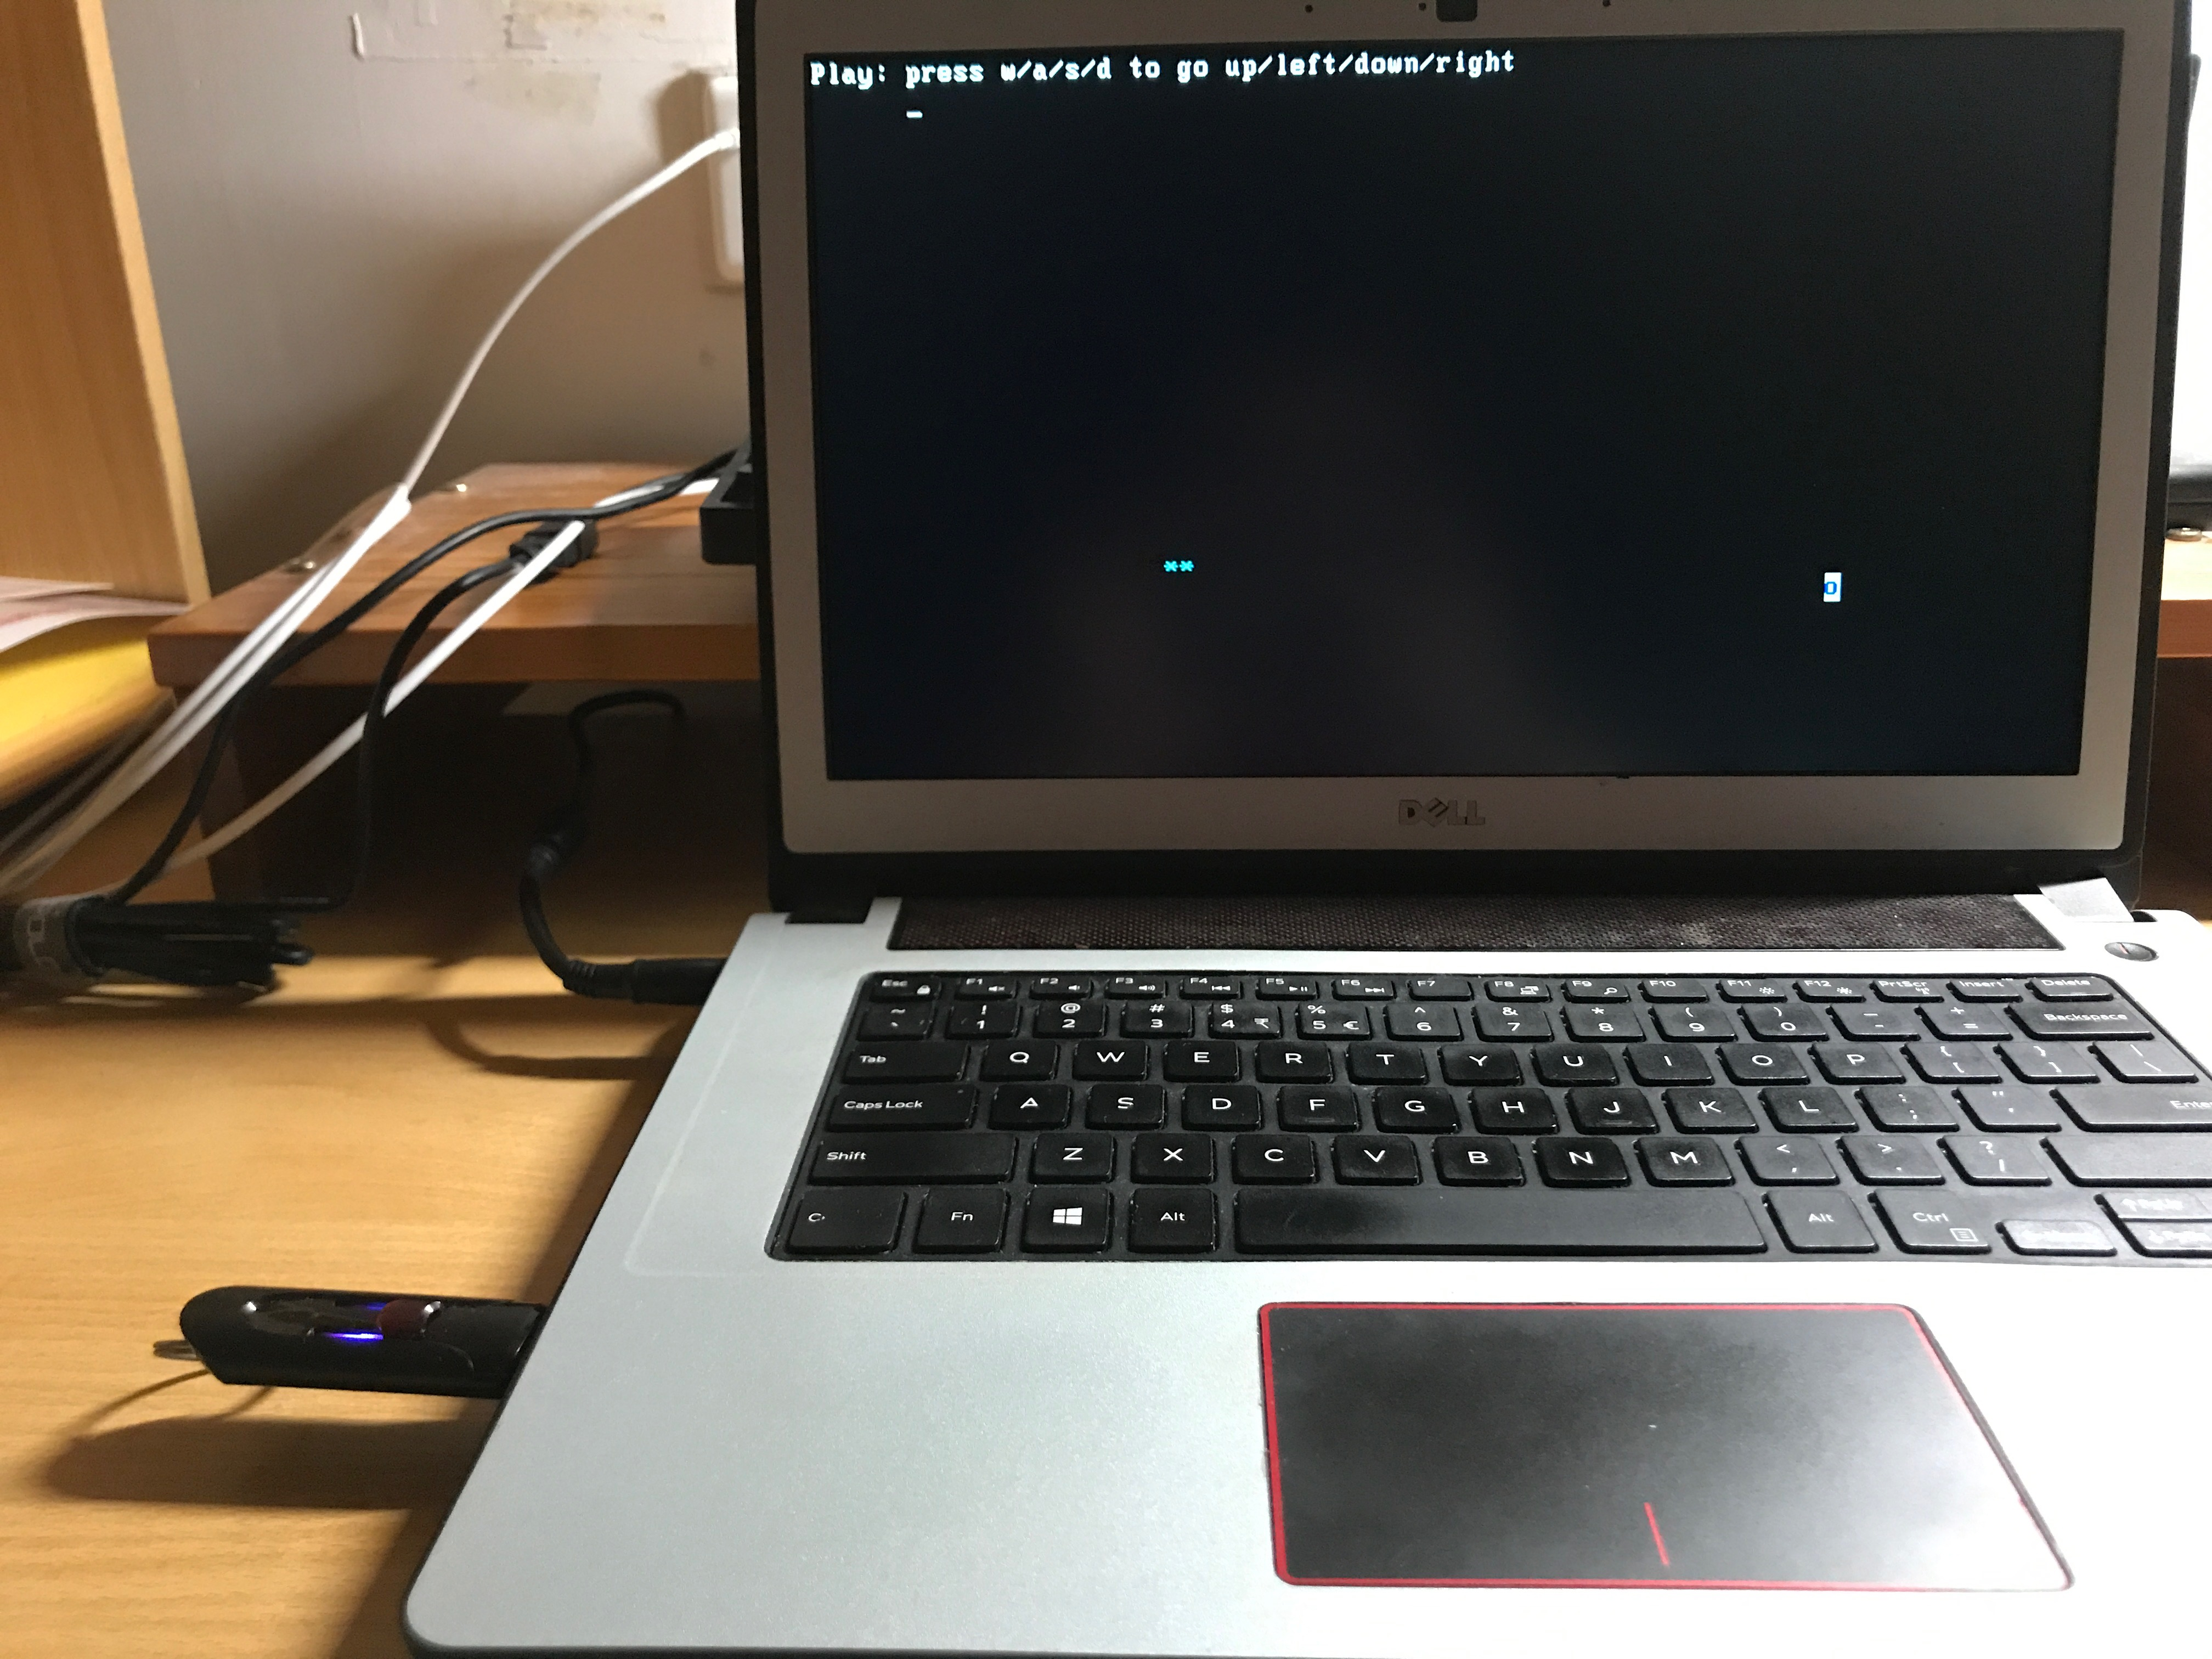
\includegraphics{/Users/lixinrui/onedrive/Documents/大学课程/2018操作系统实验/os_lab2/report/real.jpg}
\caption{}
\end{figure}

\hypertarget{header-n246}{%
\subsection{六、参考文献}\label{header-n246}}

{[}1{]}. Nasm Documentation, \url{http://www.nasm.us/doc}

{[}2{]}. GNU Make Documentation,
\url{https://www.gnu.org/software/make/manual/}

{[}3{]}. Phoenix BIOS 4.0 User's Manual,
\url{http://www.esapcsolutions.com/ecom/drawings/PhoenixBIOS4_rev6UserMan.pdf}

{[}4{]}. Ascii Table, \url{https://www.asciitable.com/}

{[}5{]}. PSP - DOS Program Segment Prefix Layout,
\url{http://stanislavs.org/helppc/program_segment_prefix.html}

{[}6{]}. C Calling Convention and the 8086,
\url{http://ece425web.groups.et.byu.net/stable/labs/StackFrame.html}

\end{document}
